\section{JaxARC as an RL Environment}\label{sec:jaxarc_environment}
% Purpose:
% Explain the parts of JaxARC that matter scientifically for the benchmark.
%
% Focus on:
% - accelerator-native execution;
% - support/query task structure;
% - access to true hidden targets for correct scoring;
% - subset/dataset coverage;
% - sweep-friendly, reproducible logging.

Turning the Abstraction and Reasoning Corpus (ARC) into a reinforcement learning environment is challenging. First, it has the usual algorithmic difficulties already emphasized by ARCLE, such as a large action space, sparse rewards, and strong variation across tasks \citep{leeARCLEAbstractionReasonin2024}. Second, it isn't a standard Markov decision process where an agent simply navigates a continuous, static world. Instead, it is a massive collection of few-shot adaptation tasks. An agent must look at a few support demonstrations, deduce a hidden geometric or logical rule, and apply that rule to a novel query grid. Furthermore, grid geometries vary wildly across tasks, ranging from $1 \times 1$ to $30 \times 30$. Moreover, the number of support and query pairs differs across tasks, and correct evaluation depends on keeping held-out targets available for scoring without exposing them to the policy.

Building a fast, JAX-native simulator for this domain requires carefully mapping ARC's highly variable, meta-learning structure into the rigid, statically-shaped constraints of compiled accelerator code. JaxARC achieves this through a functional, stateless architecture that keeps both the environment and the policy executing entirely on the GPU.

\subsection{System organization}

JaxARC uses a strictly separated architecture to keep execution fast and modular. ARC-style JSON tasks are parsed once, named subsets are resolved, and the resulting task families are packed into a fixed-shape JAX buffer on the accelerator. The compiled core of the environment then operates purely on explicit \texttt{EnvParams}, \texttt{State}, and canonical mask-based actions. 

This separation of concerns means that agent-facing wrappers—which change how policies perceive observations or parameterize actions—only alter the interface layer. They do not force the underlying simulator logic to be re-compiled. Meanwhile, exact hidden-query scoring runs in a dedicated evaluator lane, comparing the submitted terminal grid directly against the stored hidden targets without ever exposing those targets to the policy. Figure~\ref{fig:jaxarc_system_organization} summarizes this organization.

\begin{figure*}[t]
\centering
\resizebox{0.97\textwidth}{!}{\newcommand{\figstack}[1]{\shortstack[c]{#1}}

\begin{tikzpicture}[
  x=1cm,
  y=1cm,
  font=\sffamily,
  >={Latex[length=2.2mm]},
  line cap=round,
  line join=round,
  panel/.style={
    draw,
    rounded corners=10pt,
    line width=0.95pt,
    minimum height=9.70cm,
    inner sep=0pt
  },
  hostpanel/.style={panel, fill=brown!6, draw=brown!38!black, minimum width=4.80cm},
  corepanel/.style={panel, fill=blue!7, draw=blue!42!black, minimum width=6.55cm},
  evalpanel/.style={panel, fill=orange!7, draw=orange!48!black, minimum width=4.80cm},
  box/.style={
    draw=black!16,
    fill=white,
    rounded corners=6pt,
    line width=0.82pt,
    align=center,
    inner sep=6.5pt,
    font=\sffamily\scriptsize,
    text badly ragged
  },
  corebox/.style={box, draw=blue!20!black},
  supportbox/.style={box, fill=blue!4, draw=blue!32!black},
  querybox/.style={box, fill=orange!4, draw=orange!36!black},
  wrapperbox/.style={box, fill=green!4, draw=green!34!black},
  supportmetricbox/.style={box, fill=blue!3, draw=blue!24!black},
  querymetricbox/.style={box, fill=orange!3, draw=orange!26!black},
  checkbox/.style={box, fill=orange!5, draw=orange!55!black, line width=0.95pt},
  interfaceband/.style={draw=green!24!black, fill=green!3, rounded corners=9pt, line width=0.78pt},
  policybox/.style={box, fill=blue!3, draw=blue!35!black, font=\sffamily\footnotesize},
  paneltitle/.style={font=\sffamily\bfseries\fontsize{11.5}{13.5}\selectfont, text=black!92, align=left},
  panelchip/.style={draw, rounded corners=4pt, line width=0.7pt, inner xsep=5pt, inner ysep=2.5pt, font=\sffamily\bfseries\tiny},
  sidenote/.style={font=\sffamily\scriptsize, text=black!52, align=center},
  flow/.style={-Latex, line width=0.95pt, draw=blue!72!black},
  evalflow/.style={-Latex, line width=1.0pt, draw=orange!82!black, dash pattern=on 4pt off 3pt},
  legendpill/.style={draw, rounded corners=5pt, line width=0.7pt, fill=white, inner xsep=5pt, inner ysep=2pt, font=\sffamily\tiny}
]

% Panels with matched inter-column gaps
\node[hostpanel] (host) at (-6.225,0) {};
\node[corepanel] (core) at (0,0) {};
\node[evalpanel] (eval) at (6.225,0) {};

% Panel chips and titles
\node[panelchip, fill=brown!12, draw=brown!40!black, text=brown!50!black, anchor=north west]
  at ([xshift=0.34cm,yshift=-0.34cm]host.north west) {host-side};
\node[paneltitle, text width=3.95cm, anchor=north west]
  at ([xshift=0.34cm,yshift=-0.82cm]host.north west) {Offline task\\preparation};

\node[panelchip, fill=blue!12, draw=blue!42!black, text=blue!55!black, anchor=north west]
  at ([xshift=0.38cm,yshift=-0.34cm]core.north west) {compiled core};
\node[paneltitle, text width=4.10cm, anchor=north west]
  at ([xshift=0.34cm,yshift=-0.82cm]core.north west) {Compiled JAX core};

\node[panelchip, fill=orange!13, draw=orange!48!black, text=orange!70!black, anchor=north west]
  at ([xshift=0.34cm,yshift=-0.34cm]eval.north west) {evaluator};
\node[paneltitle, text width=4.10cm, anchor=north west]
  at ([xshift=0.34cm,yshift=-0.82cm]eval.north west) {Benchmark\\evaluation};

% Policy: centered to the whole figure and the core panel
\node[policybox, minimum width=4.95cm, anchor=south] (policy)
  at ($(core.north)+(0,0.58cm)$)
  {\figstack{\textbf{Agent / adaptation policy}\\PPO-style baseline or\\other task-specific learner}};

% Host column with uniform spacing
\node[box, minimum width=3.55cm, anchor=north] (sources) at ($(host.center)+(0,2.65)$)
  {\figstack{\textbf{ARC task sources}\\ \\ MiniARC, ConceptARC,\\ARC-AGI-1, ARC-AGI-2}};

\node[box, minimum width=3.55cm, anchor=north] (parsers) at ([yshift=-0.65cm]sources.south)
  {\figstack{\textbf{Parsers + named subsets}\\ \\ Normalize ARC JSON\\resolve named subsets}};

\node[box, minimum width=3.55cm, anchor=north] (buffer) at ([yshift=-0.65cm]parsers.south)
  {\figstack{\textbf{Fixed-shape task buffer}\\ \\ Padded grids + masks\\support pairs, query inputs\\stored hidden query targets}};

\node[sidenote, text width=3.60cm] at ([yshift=-0.75cm]buffer.south)
  {Built once, then reused by \texttt{reset}, \texttt{jit}, and vectorized evaluation.};

% Core column: compact and vertically aligned
\node[interfaceband, minimum width=5.90cm, minimum height=1.62cm] (iface)
  at ($(core.center)+(0,2.00)$) {};
\node[panelchip, fill=green!10, draw=green!34!black, text=green!35!black, anchor=south west]
  at ([xshift=0.16cm,yshift=0.03cm]iface.north west) {agent-facing interface};

\node[wrapperbox, minimum width=2.08cm] (actionwrap) at ($(iface.center)+(-1.6,0)$)
  {\figstack{\textbf{Action wrappers}\\point / box / flat\\to mask edits}};

\node[wrapperbox, minimum width=2.08cm] (obswrap) at ($(iface.center)+(1.28,0)$)
  {\figstack{\textbf{Observation wrappers}\\grid + optional\\input / target / context}};

\node[corebox, minimum width=4.95cm, anchor=north] (reset) at ([yshift=-0.45cm]iface.south)
  {\figstack{{\bfseries Compiled }\texttt{reset}/\texttt{step} {\bfseries core}\\sample a task and pair\\initialize the working grid and masks}};

\node[supportbox, minimum width=2.08cm, anchor=north] (support) at ([xshift=-1.35cm,yshift=-0.45cm]reset.south)
  {\figstack{\textbf{Support mode}\\visible target\\reward shaping}};

\node[querybox, minimum width=2.08cm, anchor=north] (query) at ([xshift=1.30cm,yshift=-0.45cm]reset.south)
  {\figstack{\textbf{Query mode}\\held-out input only\\target hidden}};

\node[corebox, minimum width=4.95cm, anchor=north] (state) at ([yshift=-4.25cm]iface.south)
  {\figstack{\textbf{Explicit environment state}\\working grid, input grid, target view\\clipboard, step count, task index}};

% Evaluator column with uniform spacing
\node[box, minimum width=3.70cm, anchor=north] (transition) at ($(eval.center)+(0,2.65)$)
  {\figstack{\textbf{Transition output}\\terminal grid + submit signal\\reward path + termination}};

\node[supportmetricbox, minimum width=3.70cm, anchor=north] (supportmetrics) at ([yshift=-0.45cm]transition.south)
  {\figstack{\textbf{Support-side metrics}\\success, final match\\similarity, solve steps}};

\node[checkbox, minimum width=3.70cm, anchor=north] (hiddencheck) at ([yshift=-0.45cm]supportmetrics.south)
  {\figstack{\textbf{Evaluator-only hidden-query check}\\compare the submitted grid\\against stored hidden targets}};

\node[querymetricbox, minimum width=3.70cm, anchor=north] (querymetrics) at ([yshift=-0.45cm]hiddencheck.south)
  {\figstack{\textbf{Logged query metrics}\\query success, similarity\\submission rate, truncation}};

% Interface / core arrows
\coordinate (ifacein) at (iface.north);
\coordinate (ifaceout) at (iface.south);
\coordinate (resetin) at (reset.north);
\draw[flow] (policy.south) -- (ifacein);
\draw[flow] (ifaceout) -- (resetin);

% Host internal arrows
\draw[flow] (sources.south) -- (parsers.north);
\draw[flow] (parsers.south) -- (buffer.north);

% Core internal arrows: perfectly vertical from reset to modes to state
\coordinate (resetleft) at (support.center |- reset.south);
\coordinate (resetright) at (query.center |- reset.south);
\coordinate (stateleft) at (support.center |- state.north);
\coordinate (stateright) at (query.center |- state.north);

\draw[flow] (resetleft) -- (support.north);
\draw[flow] (resetright) -- (query.north);
\draw[flow] (support.south) -- (stateleft);
\draw[flow] (query.south) -- (stateright);

% Cross-panel arrows
\coordinate (bufferblue) at ([yshift=0.20cm]buffer.east);
\draw[flow] (bufferblue) -- ++(0.55cm,0) |- (reset.west);
\coordinate (stateout) at ([xshift=0.32cm]core.east |- state.east);
\draw[flow] (state.east) -- (stateout) |- (transition.west);

\coordinate (hiddenstart) at ([yshift=-0.36cm]buffer.east);
\coordinate (hiddenlane) at ([yshift=-0.16cm]state.south);
\coordinate (hiddenelbow) at ($(hiddenstart)+(0.32cm,0)$);
\coordinate (hiddenroutea) at (hiddenelbow |- hiddenlane);
\coordinate (hiddenrouteb) at ([xshift=-0.40cm]hiddencheck.west |- hiddenlane);
\draw[evalflow] (hiddenstart) -- (hiddenelbow) |- (hiddenroutea) -- (hiddenrouteb) |- (hiddencheck.west);

% Evaluator internal arrows (centered vertical stack)
\draw[flow] (transition.south) -- (supportmetrics.north);
\draw[flow] (supportmetrics.south) -- (hiddencheck.north);
\draw[flow] (hiddencheck.south) -- (querymetrics.north);

% Legend
\node[legendpill, anchor=north, text=black!72, draw=black!20, fill=white]
  at ([yshift=0.10cm]core.south)
  {\textcolor{blue!70!black}{solid blue = simulator / policy-visible flow} \qquad \textcolor{orange!75!black}{dashed orange = evaluator-only hidden-target flow}};

\end{tikzpicture}
}
\caption{System organization of JaxARC. Offline task preparation normalizes ARC datasets and subset definitions into a fixed-shape task buffer with padded grids, masks, support examples, query inputs, and stored hidden query targets. \texttt{EnvParams} package this buffer with reward and episode-mode configuration for the compiled \texttt{reset}/\texttt{step} core, which operates over an explicit environment state. Action and observation wrappers alter only the agent-facing interface, not the underlying simulator. Support episodes expose visible targets for adaptation, query episodes mask the target in the agent-visible state, and exact hidden-query metrics are computed in a separate evaluator lane by comparing the submitted terminal grid against stored hidden targets from the task buffer.}
\label{fig:jaxarc_system_organization}
\end{figure*}

\subsection{Memory layout and the support-to-query boundary}

To make ARC compatible with JAX's \texttt{jit} compilation, JaxARC completely standardizes the memory layout. We pad all grids to a maximum $30 \times 30$ canvas and use boolean masks to track the true active area of each grid. This means JaxARC preserves ARC's original variable-size geometry functionally while keeping the memory representation statically dense. Rather than loading new data from the host CPU every episode—which creates a massive synchronization bottleneck—JaxARC preloads entire datasets into these fixed-shape PyTree buffers directly on the accelerator. 

Crucially, this memory layout enforces ARC's strict support-to-query boundary. A single task state in JaxARC bundles the support pairs, the query inputs, and the true query outputs. During support episodes, the agent can see the target grid and receive dense reward feedback to learn the rule. When the environment transitions to the query episode, it actively replaces the target grid in the agent's state with a background-colored placeholder and zeros out the target mask. The agent is forced to construct the answer blind. However, because the *true* query target (\texttt{true\_test\_output\_grids}) remains cached internally inside the environment's state, JaxARC can score the final submission instantly on the GPU. This eliminates the need to pass data back to a slow Python evaluation script, ensuring that scoring is both fast and mathematically rigorous.

Figure~\ref{fig:jaxarc_task_view} illustrates this task structure. Support pairs are presented with both inputs and outputs visible, while the held-out query is presented with its output hidden.

\begin{figure}[t]
\centering
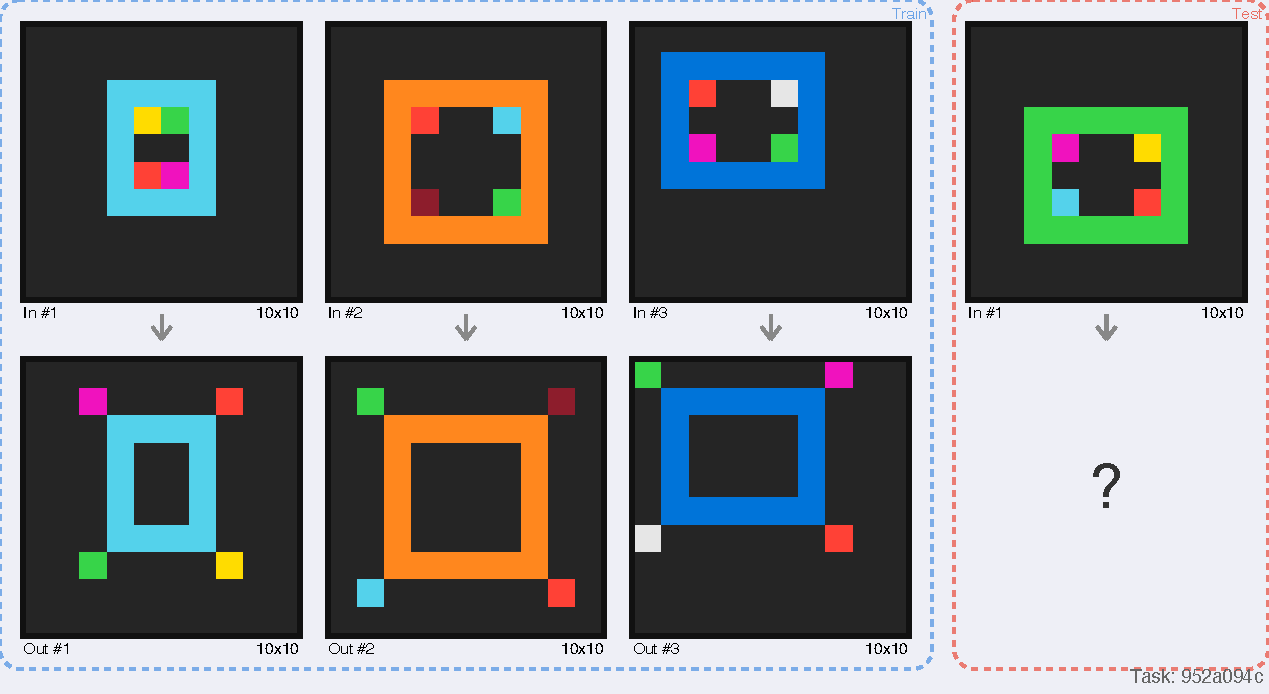
\includegraphics[width=0.98\linewidth]{Figures/viz_complete_task.pdf}
\caption{Task-level view in JaxARC. Support pairs are available as input-output demonstrations. The held-out query is presented without its target output. The policy interacts only with the visible grids; the true query target is retained internally for exact scoring of the submitted grid.}
\label{fig:jaxarc_task_view}
\end{figure}

\subsection{Mask-based editing and observations}

Previous RL implementations of ARC, such as ARCLE, modeled a rich, mutable state machine with hidden selection modes. We deliberately avoided this. JaxARC relies on a purely functional, mask-based action space. The base environment accepts an operation identifier—chosen from 35 distinct edits, including flood-fills, rotations, movements, and color swaps—alongside a binary mask that specifies exactly where to apply the edit. By keeping the core transition logic mask-based, we ensure the semantics of each action remain completely explicit in the state transition. The environment does not rely on hidden mode switches to interpret subsequent actions.

Because generating a full $30 \times 30$ binary mask is difficult for standard policy networks, we provide lightweight wrappers to simplify the agent-facing action space. A point-action wrapper reduces the output to a simple $(\text{row}, \text{col}, \text{operation})$ tuple, converting that selection into a mask under the hood. A bounding-box wrapper similarly lets the agent select rectangular regions. A flattening wrapper can even collapse composite discrete spaces to guarantee compatibility with standard discrete agents. 

The observation side mirrors this flexibility. The base observation is just the current working grid. Optional wrappers allow researchers to append the original input grid, the clipboard state, the visible target grid, or contextual support pairs from the same task. This separation lets researchers vary the interface available to the agent without changing the task semantics or evaluation logic underneath.

\subsection{Rewards and diagnostics}

The true objective in ARC is sparse and submit-based: the agent only succeeds if its final submitted grid is a perfect, pixel-for-pixel match with the target. JaxARC explicitly implements this exact-match objective, awarding a success bonus only when the agent formally submits and the similarity reaches 1.0. 

Because pure sparse rewards are nearly impossible to optimize from scratch, the environment also exposes configurable shaping. During support phases, researchers can enable dense rewards based on intersection-over-union (IoU) similarity, as well as step penalties or penalties for invalid submissions. Crucially, this shaping is disabled during hidden-query evaluation to prevent the agent from "guessing" the answer via reward gradients.

Beyond scalar returns, JaxARC tracks detailed episode diagnostics: whether the agent submitted an answer, whether the episode truncated due to time limits, the best similarity achieved, and the exact similarity score of the final grid. ARC failure is not one-dimensional. An agent might perfectly replicate the support grid but fail to submit, or it might submit more frequently on hidden queries without ever being correct. JaxARC logs these distinctions explicitly so researchers can understand exactly how an adaptation strategy is failing rather than just observing a zero return.

\subsection{A unified pipeline across datasets}

Finally, JaxARC standardizes the environment surface across MiniARC \citep{kimPlaygroundsAbstractionReasoning2022}, ConceptARC \citep{moskvichevConceptARCBenchmarkEvaluating2023}, and the canonical ARC-AGI-1 \citep{cholletMeasureIntelligence2019} under a single API. This provides a clear, escalating pipeline for research. Teams can prototype architectures on the fast, simplified MiniARC tasks, diagnose specific algorithmic failures on ConceptARC's isolated cognitive skills, and run final evaluations on canonical ARC tasks, all without changing a single line of environment code. 

Ultimately, JaxARC is more than just a fast simulator. By formalizing ARC's highly variable task structure, enforcing strict hidden-query evaluation, and providing controlled agent interfaces, it creates an accelerator-native foundation that makes large-scale, compute-budgeted adaptation studies genuinely practical.